% This file is isea.tex. It contains the formatting instructions for and acts as a template for submissions to ISEA 2025. It is based on the ICCC formats and instructions. It uses the files isea.sty, isea.bst and isea.bib, the first two of which also borrow from AAAI IJCAI formats and instructions.
% Modified from ICCC.tex by B. Bogart

\documentclass[letterpaper]{article}
\usepackage{isea}
\usepackage[pdftex]{graphicx}
\usepackage{times}
\usepackage{helvet}
\usepackage{courier}
\usepackage[numbers]{natbib}
\pdfinfo{
/Title (Towards an Effective Theory of Art)
/Author (Kynan Stewart Hughes)}
% The file isea.sty is the style file for ISEA 2025 proceedings.
%
\title{Art as Technology v0.1.1}
\author{Author: Anonymous\\
School: Anonymous\\
Institution: Anonymous\\
Location: Anonymous\\
Email: Anonymous\\
% \author{Kynan Stewart Hughes\\
% Creativity and Cognition Studios\\
% University of Technology Sydney\\
% Sydney, Australia\\
% kynan.s.hughes@student.uts.edu.au\\
\newline
\newline
}
\setcounter{secnumdepth}{0}

\begin{document} 
% Setting the default tolerance level
% \tolerance=200
% Setting a high tolerance level
% \tolerance=10000
% Some more drastic measures for hbox issues
% \emergencystretch=4em
% \raggedright
\maketitle
\begin{abstract}

This paper examines the conceptualisation of art as a technology, drawing on theories from complexity science and process philosophy to explore how art objects function to produce meaning. The discussion reveals how art captures the observed regularity of human capacity for affect, deploying it to reorder information and generate indeterminate contextual networks. This view positions art within a broader continuum of crafting, challenging the divide between artistic and technical domains, and suggesting that art might be seen as an expressive technology embedded in an ethics of interconnectedness.
\end{abstract}

\keywords{Keywords}

Art, technology, complexity, aesthetics, affect, information, craft, systems, emergence, meaning, constraints, coarse-graining

\section{Introduction}

    %The notion of art as a form of technology opens pathways for understanding how art functions beyond traditional aesthetic or expressive categories.  
    % In the lexicon of Deleuze and Guattari technical \emph{machines} are a subset of the larger set of productive assemblages that constitute the world, but 
    There is a sense in which the term \emph{machine} is used in some of the recent literature about art that is bordering on technological. In \emph{Art As Abstract Machine}, Stephen Zepke, quoting Giles Deleuze, announced that 

    \begin{quote}
        [...] art as abstract machine will require an artist adequate to the task: a mechanic. For each machine its mechanic: "The painting machine of an artist-mechanic." \citep[p.1]{ZepkeArtAsAbstrctMchn2005}
    \end{quote}

    With this metaphor, Zepke was inviting the reader to play with the idea that art is a kind of technology. Simon O'Sullivan has gone a little further. In reference to Deleuze's concept of \emph{the virtual}, he has suggested that “it might be useful to [...] understand art as operating as a kind of ’actualising machine‘” \citep[p.200]{ZepkeOSullivanDlzCntmprryArt2010}, and has called art an “aesthetic event-based technology” \citep[p.202]{ZepkeOSullivanDlzCntmprryArt2010}. Anne Sauvagnargues has drawn parallels between Deleuze’s ideas on art and Gilbert Simondon’s concept of the technical object, suggesting that art operates as a specific kind of technology, one that modulates forces and generates meaning \citep[pp.74-75]{SauvagnarguesArtmchns2016}.

    This paper examines how art might function, technically, by capturing our evolutionary capacity for aesthetic experience and deploying it to create meaning. The aim is not to prescribe fixed conclusions but rather to stimulate inquiry into how this conceptual shift might reshape our understanding of art's role and potential.

    The analysis is grounded in complexity thinking, a meta-theory applicable to any dynamic system, including art and technical objects \citep{CilliersRichardsonCmplxtyScnc2001}. In science, the rapid development of complexity thinking over the last several decades, including Chaos Theory, Dynamical Systems Theory, and Complex Adaptive Systems Theory, is a paradigm shift from deterministic models to a view that embraces the interdependent, adaptive, and emergent nature of systems. This paper draws on concepts from complexity science and Process Philosophy, revealing a framework in which art as technology, operates as a complex system of affect, information, and meaning.
    
\section{Technology}

    According to Brian Arthur a technological object is always “a phenomenon captured and put to use” \citep[p.53]{theNatureOfTechnology2009} or, putting it another way, “a programming of phenomena for a purpose.” \citep[p.53]{theNatureOfTechnology2009}. This distillation holds for the full range of diverse technologies, contemporary and historical.

    Phenomena don't have to be physical phenomena like fire or electricity. They may be “behavioural or organisational ‘effects’” \citep[p.55]{theNatureOfTechnology2009} or “truism[s] of nature” \citep[p.45]{theNatureOfTechnology2009}. We might update Arthur's definition of technology by applying biologist and complexity scientist Jessica Flack's concept of \emph{course graining} in place of the more fuzzy idea of “phenomena”. 

    According to Flack, \emph{coarse-graining} occurs when a subsystem with apparently emergent properties is treated as a single entity by components of the system for predictive purposes. Course graining is a way of reacting to another element of a complex system that works but ignores many of the details. It is “lossy but true” \citep[p.4]{FlackCrsGrnng2017}.

    \begin{quote}
        Having a basis in mechanism is a critical property of a coarse-grained description — it is “true” to the system. It is a simplification of the microscopic details. In principle, a coarse-grained description does not introduce any outside information to the subset of microscopic interactions over which it is performed [...] \citep[p.4]{FlackCrsGrnng2017}
    \end{quote}

    Flack has used the idea of temperature\footnote{

        Flack has remarked that this example comes from \emph{Inventing Temperature} by Hasok Chang \citep{ChangInvntngTmprtr2004}

    } as an example of the kind of coarse-graining scientists do.

    \begin{quote}
        Temperature is the average speed of particles in a system. Temperature is a coarse-grained representation of all of the particles” behaviour — the particles in aggregate. When you know the temperature you can use that to predict the system's future state better than you could if you actually measured the speed of an individual particle. Temperature can predict the future state of the system (assuming it is at equilibrium) more computationally efficiently because it requires fewer degrees of freedom. \citep[p.4]{FlackCrsGrnng2017}
    \end{quote}

    Apparent phenomena in complex systems are always the result of coarse graining. Course-graining is a concept that describes how emergence happens — or at least something about its necessary conditions. A property like temperature emerges, through processes that include course-graining, from interactions between physical substances, people measuring, systems and devices of measurement, and the environment. A distribution of relative status ‘scores’ in a monkey group emerges, through processes that include a very similar kind of coarse-graining, from a system of signalling interactions between individual monkeys and the perception of those signals by the group. The same processes play out in coral reef formation \citep{FlackEtAlTmsclsSymmtryUncrtnty2013}. Even something apparently as straightforward as the emergent properties of an instance of metal alloy require, to be realised, a system of things that interact with the instance as a whole and not just as a collection of atoms.

    We might say then, that a technological object is \emph{the programming of observed regularity for a purpose}.

    A monetary system, for example, is a technology because it depends on an observed regularity of human behaviour.

    \begin{quote}
        The monetary system makes use of the “phenomenon” that we trust a medium has value as long as we believe that others trust it has value and we believe this trust will continue in the future. \citep[p.55]{theNatureOfTechnology2009}
    \end{quote}

\section{The Aesthetic Regime of Art}

    Jacques Rancière has called the current regime of art, art as we know it, the \emph{aesthetic regime}.  It is not a single coherent paradigm, but a “plurality” of “frequently different, and sometimes contradictory, ways of thinking” \citep[p.8]{RanciereMdrnTms2022} organised around the idea of aesthetic experience (a radical repositioning of Aesthetics as art itself, rather than as a theory about art).
    
    The aesthetic regime emerged at the end of the eighteenth century with Emanuel Kant's \emph{Critique of Judgement}. Kant's radical break was to propose that the essence of an art object lies in its capacity to be experienced without concept. With the clarity of hindsight, we can see as Rancière did, that it is the separation of sense-as-in-sensation and sense-as-in-making-sense which created our current situation in which the effectiveness of an artwork, the very thing that makes it art, is (as Rancière put it) “a paradoxical kind of efficacy that is produced by the very rupturing of any determinate link between cause and effect.” \citep[p.51]{RancierThEmncptdSpcttr2009} ”It is precisely this indeterminacy”, he said, “that Kant conceptualized when he defined the beautiful as ‘what is represented as an object of universal delight apart from any concept’. \citep[p.52]{RancierThEmncptdSpcttr2009}

    The purpose of an artwork (we might call it \emph{meaning} since they amount to the same thing for artwork) is always organised around aesthetic experience. This constraint is the origin of art's autonomy within Modernity and the source of all possibility with respect to how art can interact with other aspects of Modernity, including all potential for generating meaning or taking political action, for example. All distinctions and differences within the idea of art operate within the aesthetic regime. Ideas about Modern and Post-Modern art, for example, are simply different, perhaps contradictory strategies for trying to do something worthwhile within the aesthetic regime \citep[p213]{ZepkeSblmArt2017}. Art which is anti-aesthetic is still operating within the aesthetic regime in a way that is self-consciously critical of it — in fact, because of that. Conceptual art invites us to consider the aesthetic potential of ideas.

    One of the key features of the aesthetic regime, according to Rancière, is that it enables objects created under other regimes — for purposes other than aesthetic appreciation — to be experienced as art. As Marcel Duchamp proved in 1917 when he entered a urinal into an art exhibition, and as has been proven many times since by practitioners of Contemporary Art for whom the readymade is a key strategy, there is nothing in the world that cannot be made into a work of art even by the simple act of declaring it to be one. A kind of transfiguration, or dislocation, occurs when an object is brought into the aesthetic regime. The object is no longer understood in terms of its original function or purpose, but as an object of contemplation within the aesthetic regime. “The aesthetic regime”, as Rancière put it, “asserts the absolute singularity of art and, at the same time, destroys any pragmatic criterion for isolating this singularity. It simultaneously establishes the autonomy of art and the identity of its forms with the forms that life uses to shape itself.” Literally anything can be art. It is not simply that objects \emph{can} be transfigured into art objects, but that the aesthetic regime \emph{is} a system of codes that dislocates objects from their original functions and meanings. This “dissensual operation” of creating an artwork, for example by working materials into forms, by organising sounds in certain ways, by setting the state of pixels on a screen, by isolating and performing specific movements with our body, or by repurposing a ready-made object, “transforms a given form or body into a new one.” \citep[p.54]{RancierThEmncptdSpcttr2009}.

    The aesthetic regime may be Modern, aesthetics powered art machine, but it is housed in the somewhat clunky vestiges of two older regimes. 
    
    The aesthetic regime is directly superimposed upon (without replacing) the previously dominant \emph{regime of representation}. The idea of there being a qualitative difference between the practices we now call ‘the arts‘ and other technologies began taking shape during the Renaissance \citep[p.136]{TatarkiewiczWhtIsArt1971} and by the late 17th century the classification of various practices within this category of ‘the arts’ had become a hot topic in European intellectual circles.

    According to Rancière, the plane on which this qualitative difference emerged, the principle that came to organise these ‘ways of doing, making, seeing, and judging’, this ‘fold in the distribution of ways of doing and making’, was the ‘notion of representation or \emph{mimesis}’. He called this partitioning of the sensible the \emph{regime of representation} \citep[p.22]{RancierPltcsOfThAsthtcs2004}. It is not, in itself, an artistic process, but ‘a fold that renders the arts visible.‘ It is  ‘a regime of visibility regarding the arts.’
    
    Although the various \emph{arts} existed — understood as forms of knowledge and their applications — they were not recognised as part of a singular, overarching category of human experience called “art”. The arts — music, literature, sculpture, painting, et cetera — were disparate practices serving different social functions, and were situated within a stratified system that categorised both activities and the individuals engaged in producing them. The concept of art as a unified field was absent. Also, everything made sense. The job of the arts was to represent the world as a unity of sensible order. A place for everything and everything in its place, including people.
    
    The aesthetic regime is strategy that creates the possibility for new ways of being in the world, cutting across the regime of representation - but we still observe the fold of difference that separates the arts from the non-arts. For example, we organise our institutions of learning — our university faculties and school curriculums — along it: science, technology, engineering and maths on one side, the arts and humanities on the other. We wonder how to get more girls to choose STEM subjects in school. It is this fold in the distribution of the sensible that the idea of art as a technology smooths out. But what would it be like for this fold not to exist? Is an alternative even possible?

    Heidegger, in his essay \emph{The Question Concerning Technology}, pointed out that ‘techne’ was the Greek word for skill, craft, and technique\footnote{Reference needed.}. The term covered what we might now call ‘the arts’ as well as the sciences, and the technologies which seem archaic to us now and which we call ‘crafts’. The idea of art did not exist as a separate category of making within this field. For Plato, for example, ‘art’ did not exist, but only ‘arts’, ways of doing and making \citep[p.20]{RancierPltcsOfThAsthtcs2004}. Plato had opinions about the relative merits of the various arts. There are, he thought, true arts, which are forms of knowledge based on the imitation of a model with precise ends, and lesser arts that simply imitate appearances \citep[p.20]{RancierPltcsOfThAsthtcs2004}.  Rancière has called the mode of thought that governed the kinds of activities we now associate with artmaking back in ancient times, when art, science, technology et cetera were all simply different kinds of crafting, the \emph{ethical regime of images}:

    \begin{quote}
        In this regime, ‘art’ is not identified as such but is subsumed under the question of images. As a specific type of entity, images are the object of a twofold question: the question of their origin (and consequently their truth content) and the question of their end or purpose, the uses they are put to and the effects they result in. The question of images of the divine and the right to produce such images or the ban placed on them falls within this regime, as well as the question of the status and signification of the images produced. The entire Platonic polemic against the simulacra of painting, poems, and the stage also falls within this regime. [...] In this regime, it is a matter of knowing in what way images' mode of being affects the ethos, the mode of being of individuals and communities. This question prevents ‘art’ from individualizing itself as such. \citep[pp.20-21]{RancierPltcsOfThAsthtcs2004}
    \end{quote}

    Like the regime of representation, the ethical regime of images didn't go anywhere — it is very much still an aspect of the way we \emph{partition the sensible}, as Rancière has labelled the largely unconscious sensemaking processes in and with which humans are constantly engaged. We still care about who produces what images and for what purpose, as well as the potential effect images have on society. In Australia in 2008, an exhibition by the well established artist Bill Henson was shut down by police after complaints that his artworks contained the images of naked children. Many people fear that AI generated imagery is undermining the truth value of images and are being used to manipulate people. Graphic artists, illustrators and photographers complain about the proliferation of AI generated images that can mimic their style and affect the market for their work. The ethical regime of images is still with us, and it forms part of how we think about art. 

    Techne didn't disappear either. Instead of ‘techne’, which sounds a bit archaic, I'm inclined to use the English word ‘crafting’ — and I'm thinking here about how the word is used in the context of the open-world game Minecraft, as a kind of basic human activity, a kind of compulsion to make things. The concept of crafting can be equally well applied, in a contemporary context, to art, to the arts (music, writing, etc.), to traditional crafts and also to the newest technologies. Perhaps it doesn't apply so seamlessly to scientific practices, but even scientists can craft compelling arguments, elegant experiments and sound theories.

    ‘Crafting’ implies a sense of purpose more than does, say, the more general term ‘making’. A sea snail moving across the sand ‘makes’ a trail but the trail, at least for the snail, has no purpose and we wouldn't say that the snail ‘crafted’ the trail. A bird, on the other hand, makes a nest for a purpose, and we might very well describe this activity as crafting. A bowerbird crafts a bower for the purpose of attracting a mate and establishing a territory in which certain rituals of courtship can take place. Deleuze and Guattari suggested that human artmaking has its origins in the kinds of territorialising activities animals perform \citep[p.15]{GuattariChsmss1995}. Crafting is baked into us. We are the animals who have taken crafting to an extreme.

\section{Affect}

    For Kant, the range of aesthetic experience as it pertains to art objects was limited to the experience of beauty.  He also, at the last moment, included ‘the sublime’ \citep[p.15]{ZepkeSblmArt2017} as that which is experienced as a kind of rapid toggling back and forth between fear and pleasure — an awe-inspiring natural scene, for example — but he didn't consider this to be the kind of experience one can have with an artwork\footnote{Reference needed.}. The exclusive focus on beauty is starting to seem like a strangely unnecessary limitation to put on aesthetic experience and on art. 
        
    The concept of \emph{affect}, which comes from Deleuze and Guattari via Brian Massumi, is a way of thinking about how things affect other things in complex systems of interconnections that is the world, including the way that our bodies and minds are affected by the world around us. Affect is a kind of intensive interaction that is not yet a feeling. Affect is always also going on all around us. It is in no way limited to being human. It is human and inhuman, organic and inorganic. It is the way that we and things are moved by the world and each other, and it is also a kind of pre-cognitive, pre-linguistic, pre-conscious event during which the world emerges into existence. 
        
    Contemporary scholars, coming at aesthetics from the perspective of affect, note that the field of Aesthetics had been developing for 40 years or so before \emph{Critique of Judgement} was written and that its remit was more broad than experiences of beautiful, or even sublime, art. The inception of aesthetics as a field is attributed to European philosopher Christian Wolff and his disciples, including Moses Mendelssohn and, especially, Alexander Baumgarten \citep[pp.327-338]{EagletonFrPrtclrs1990}. Baumgarten thought that the Cartesian philosophical emphasis on logic and conceptual thought had neglected the epistemological role of sensorial experience. For him, aesthetic cognition mediated between reason and sense; the aesthetic was a kind of (inferior, feminine) analogue of reason, operating at the level of material life. 
        
    The entangled dualism that aesthetic experience should be mainly limited to experiences of art and that these experiences should be limited to beauty, possibly with a kind of partial dispensation granted to the sublime, now seems naive. Ben Highmore, in the context of arguing for a more expanded view of aesthetic experience as synonymous with affect, has pointed out the historical logic connecting beauty and art as a morally uplifting activity \citep[p.121-122]{HighmoreBttrAftrTst2010}. Baumgarten thought that, within the dense amorphous flow of our sensuous experience constantly in flux, certain objects stand out in a kind of ideality akin to rational perfection, which is beauty \citep[p.328]{EagletonFrPrtclrs1990}. It makes sense, Highmore suggests, that beauty should become the approved affective experience for art objects, because art was a kind of moral training for the soul, and beauty was the most morally uplifting affect.
        
    The recent move to equate aesthetic experience with affect is a shift away from the idea that some normative experiences are better than others and that the artwork is a moral lesson, and towards the messy reality of material processes. It contextualises aesthetic experience in a complex ecology of affect. As Highmore put it, referencing Guattari, art is now about “complex affective and intensive exchanges, situated in the broader ecology of the world.” \citep[p.155]{HighmoreBttrAftrTst2010}

    A male bowerbird crafts a bower, so as to generate affect in a female bowerbird for the purpose of mating. If, as Deleuze and Guattari suggested, human artmaking has its origins in theses kinds of activities, then surely we are unique in the extent to which we craft objects designed to generate affect.
    
    The aesthetic regime is a kind of system of codes that dislocates objects and materials from their original functions and meanings, and imbues them with affective potential. It is essentially a hack on our capacity for affect.

\section{Purpose, Meaning and Information}

    Jason Hoelscher has argued that art, as a system of practice theory, is a complex adaptive system \citep[p.38]{HoelscherNtsOnAtctlytcAsthtcs2015}. It uses the concept of dynamic equilibrium to describe the balance between the drive for novelty and the gravitational pull of established patterns or “attractor basins” within this system \citep[pp.41-42]{HoelscherNtsOnAtctlytcAsthtcs2015}. This balance ensures that while art is perpetually evolving, it remains anchored within a broader discourse, allowing for the formation of information-entropic dissipative structures — artworks. These objects, rich in complexity and depth, invite continuous interpretation and re-interpretation, reflecting the co-evolutionary nature of artistic practice and theory as they adapt and respond to each other and to their changing contexts. 
    
    Hoelscher has also referred to art styles and to recurring motifs in art as attractors. For example:
    
    \begin{quote}
        [...] the human figure constitutes an artistic attractor of great power and draw, being “an oscillatory limit cycle around which the system flows repeatedly” (Kauffman 1993, 176) \citep[pp.11-12]{HoelscherThPtcsOfPhsSpc2014}
    \end{quote}

    Artworks are indeterminate in that meanings are not fixed. The shifting meanings attributed to art objects over time and in different contexts are “a series of attractor basins in possibility space” \citep[p.4]{HoelscherThPtcsOfPhsSpc2014}
    
    \begin{quote}
        Being unfinalizable and open, and manifest via the tautology of purposiveness without purpose, an artwork draws the viewer toward possible interpretations while nonetheless preventing a fixed, final understanding. It is this epistemological opening around which the artwork-as-attractor basin accretes, around which a swarm of interpretations are possible but never definitively attained. \citep[p.12]{HoelscherThPtcsOfPhsSpc2014}
    \end{quote}

    Information is for complexity science what energy is for classical physics\footnote{Reference needed - Crutchfield} Information is central to Hoelscher's theory of art. He has blended Claude Shannon's Information Theory with Gilbert Simondon's idea of information as arising from meaningless disparity as emergent, meaningful difference. Hoelscher summed up Simondon's concept of information as “relational operation of difference that intensifies or generates a context”. He has described art objects as a sources of information because they are open to interpretation — that is, they are interpreted relative to a context. 
    
    Hoelscher has reminded us that information was shown by Shannon to be a function of the relative entropy of a system — that is, the total available entropy (all the possible states of a system in a given context) minus the actual entropy (the actual state of the system). He has pointed out that entropy is a form of symmetry, using the example of a white cue ball as an example of an object that is symmetrical with respect to rotation.
    
    \begin{quote}
        [...] Entropy is a form of interchangeability. Interchangeability is another word for an extreme degree of symmetry: the white cue ball can be rotated, rearranged, flipped, and so on without notable difference in appearance, because its surface areas are extremely symmetrical and interchangeable — entropic, in other words.
    \end{quote}

    Since “information for Shannon is a measure of the surprise, or difference from expectation, created when a difference emerges into, or travels through, a context” \citep[p.6]{HoelscherArtAsInfrmtn2021}, with respect to changes in rotation there is no information in this cue ball system. 
    
    However, where there is a lack of symmetry, there is information. We might imagine a cue ball that suddenly develops a single protruding bump. Now, relative to rotation, the system is not symmetrical. This would be an entirely new system in which information is possible. As Hoelscher points out, “information for Simondon is a relational operation of difference that intensifies or generates a context” \citep[p.6]{HoelscherArtAsInfrmtn2021}. 

    The resolution of meaningless disparity into meaningful difference is a wildly creative act that results in an exponentially more vast field of potential for meaningful action — a huge increase in capacity to affect and be affected. Hoelscher has invited us to consider, for example, the evolution of eyes from, perhaps, light-sensitive areas on an organism's surface, that eventually become sensitive enough to allow the creature to perceive (on some unconscious level) a consistent (regular) difference in the input signal from different eyes. Suddenly, in the macro-scale equivalent of a quantum shift, a three dimensional universe comes into existence.

    \begin{quote}
        This slight distance between one eye and the other causes two distinct visual streams, which resolve into the rich depth perception of binocular vision. Here, the reconciliation of a simple disparity yields a result far more complex than one might expect, given the small scale of the initial problem. \citep[p.5]{HoelscherArtAsInfrmtn2021}
    \end{quote}

    Since an art object never settles into one particular, fixed state of communicated meaning, it is an open-ended, endlessly generative source of information \citep[p.7]{HoelscherThPtcsOfPhsSpc2014}. As Hoelscher has explained it, art is tapping into the generative power of the universe itself, which is always creating information.

    \begin{quote}
        I believe this asymmetry creates a high degree of preinformational directionality — a highly charged, saturated and unstable disparity that “wants” transductively to be discharged. Relative entropy thus contains a core element of self-differencing — as a range of potential options and occasional actualizations, the universe seems unable to do anything \emph{other than to create information}.
    \end{quote}

    Art itself is constantly evolving, generating new styles and discourses that increase the range of possible interpretations and creative options.

    \begin{quote}
        [...] Each new stylistic and discursive development [...] increases the range of options available for future stages of artistic change while decreasing the ability to predict still further changes due to the increase of available options. In information theory terms, then, each such expansion increases the range of signal unpredictability — and thus information content — still further, creating an autocatalytic aesthetico-information feedback loop. \citep[p.2]{HoelscherThPtcsOfPhsSpc2014}
    \end{quote}

    Hoelscher has said that art objects are epiphenomenal, like rainbows \citep[p.17]{HoelscherArtAsInfrmtn2021}. It is always possible to see how they are the result of some other phenomena. The materials from which they are made are always visible, and yet the artwork exists somehow separately from these materials. An art object is made, in a way, out of its own \emph{artness}.
    
    \begin{quote}
        [...] a work of art is a complex adaptive epiphenomenon of its own manner of phenomenalization: the penumbra of indeterminacy around an artwork is what defines it as an artwork, and is not only the effect of its mode of instantiation but also its cause. In other words, art is a self-ramifying process, an unfinalizable feedback loop \citep[p.2]{HoelscherThPtcsOfPhsSpc2014}
    \end{quote}

    In Hoelscher's formulation, art objects are indeterminate because they are, as Kant suggested, “purposive without a purpose” \citep[p.57]{KantCrtqOfJdgmnt}. They are made but, unlike everything else humans make, their purpose is only to be art objects. 

    \begin{quote}
        The claim here is not that art lacks purpose, but that art's purpose is contextually complex and indeterminate, and so remains open to transformation and differentiation by lacking external, objectively shared criteria by which to resolutely judge or interpret the work. Lacking this anchor of specificity, art's purpose remains expansive, many layered, and multidimensional.\citep[p.25]{HoelscherThPtcsOfPhsSpc2014}
    \end{quote}

    These epiphenomenal art objects grab our attention by their virtue of their complex, contingent mode of existence.

    \begin{quote}
        An epiphenomenon thus foregrounds its existence not as a resolute or finished thing but as the ongoing operational contingency of itself, as itself. Whether in the guise of a rainbow or an artwork, the strangeness of this perceived contingency — of a sustained process of focused incompletion taking place right before our eyes — compels us to stop, look, and linger.
    \end{quote}

    Once they have our attention, these “differentially complex” \citep[p.74]{HoelscherArtAsInfrmtn2021} objects make information available that is otherwise hidden in plain sight as apparently disordered, entropic chaos.
    
    Far from being a non-ordered type of entropy, the disorder of the world is “a highly charged and catalytic mode of entropy akin to information entropy — not inert, but saturated to bursting with potentials that are oriented toward actualization.” \citep[p.72]{HoelscherArtAsInfrmtn2021}. Disorder, he says quoting Henri Bergson, “is simply an order we are not looking for.” \citep[p.73]{HoelscherArtAsInfrmtn2021}. Within this milieu, potential orderings “bustle and crackle”, awaiting “catalytic discharge upon their convergent processing through the differential gap.” \citep[p.73]{HoelscherArtAsInfrmtn2021}, which “sheds information that shows up as a difference that makes a difference.” \citep[p.75]{HoelscherArtAsInfrmtn2021}. Helpfully, Hoelscher provided a number of examples.

    One example is the hyper minimalist sculptures of Robert Morris, which are simple grey cube-like forms placed directly on the floor of a gallery.

    \begin{quote}
        By giving the viewer so little to look at, Morris [...] directs the flow of attention away from the object itself and toward the object's relations with the gallery space, with the changes of light and shadow over time, and with the viewer's field of experience as an experience in and of itself. Accordingly, with the severe reduction of the work's surface qualities, internal differentiations, particularity, and variability, the artwork and its local situation fold into one another — a direct ingression of the differential information object into the space of lived experience. \citep[p.78]{HoelscherArtAsInfrmtn2021}
    \end{quote}

    Another example is a Duchamp readymade. Describing \emph{In Advance of the Broken Arm} (a snow shovel) Hoelscher said:

    \begin{quote}
        [...] the readymade's enfolding of object and idea activates (and is activated by) a wide-ranging network of differential tensions between the object and its context, and between cultural, historical, and artistic expectations regarding shovels, artworks, and the application of artistic skill [...]
    \end{quote}

    This is nothing we haven't heard before with respect to a Duchamp readymade. What is interesting is that it is another example of existing information reordering around an art object. In this case the information is very different from that which reorders around a Morris sculpture. The Morris sculpture reorders information around the object's relation to the gallery space, light and shadow, and the viewer's experience. The Duchamp readymade reorders information around the object's relation to the history of art, the history of shovels, and the history of Duchamp's own work. The information that is reordering is different, but the process is the same.

    Alicia Juarrero's concept of \emph{enabling constraints} is especially useful as a way to think about meaning because it gives artists something to grab onto.  Drawing heavily on the idea of \emph{redundancy} from Shannon's Information Theory, Juarrero has identified two types of constraints that define the probability space of complex systems: context-free constraints and context-sensitive constraints. In terms of information, both types of constraints are necessary for reducing randomness in order to separate information from noise but, she says, only context-sensitive constraints enable signals that convey meaning. While both types of constraints function by limiting possibilities, context-sensitive constraints also create possibility by connecting a simple message/information system that is initially defined by context-free constraints with the complex systems in which it is embedded. Context-sensitive constraints explain emergence.

    \begin{quote}
        Contextual constraints operating "bottom up" (as "enabling constraints") are responsible for the formation of higher level wholes with emergent properties. \citep[p.240]{JuarreroCsltyAsCnstrnt1998}
    \end{quote}

    Context-free constraints are the traditional idea of a constraint such as can be found in mechanics. They simply limit the potential states a system can be in. Context-sensitive constraints limit the system's state space as well, but they also create new dimensions of possibility by connecting the system with the state-spaces of other systems. Context-sensitive constraints may be analogous, to some extent, with the idea of a system's control-space. They explain how complex phenomena, like life happen. 
    
    Juarrero has illustrated the way enabling constraints operate using an example of a lighthouse\footnote{

        Juarrero attributes this analogy to Bob Artigiani.

    }. This is a good example for a project about artmaking because it relates directly to how meaning emerges from the interactions of components in a system.

    A lighthouse is an information channel: it is physically constrained to having only two possible states — it can only blink on and off. Without any other context — say, when it is seen by a Martian on mars — the sequence of signals from a lighthouse amounts to transmitting “Message”, “Message”, “Message”. The message contains information in the sense Shannon defined it, but it has no meaning. The meaning comes from the constraints that connect the flashing light with a broader network of things and events.

    \begin{quote}
        It is because of his awareness of a network of relationships that the sailor, unlike the Martian, can understand that the flashes of light he sees mean "Land!". The sailor sees the flash of light as a node in a complex network of relationships [...] Indeed, the sailor is a sailor (and not just a man adrift on a boat) only because he himself is embedded in a network of [contextual] relationships (such as navigation, tacking into the wind, etc). [...] Signals subject to [contextual] constraints refer to the contextual web (temporal and spatial) in which that particular signal or event is embedded. The information such signals or processes carry is of the organization of the network; the actual information content is about the overall web, not just of its components.\footnote{

            I have swapped out Juarrero's technical term “D2 type” for the more friendly “contextual” simile she uses elsewhere in the article.

        } \citep[p.237]{JuarreroCsltyAsCnstrnt1998}
    \end{quote}
    
    If we want to add more meaning to the flashing signal, we need, paradoxically, to impose more constraints on it. For example, Morse code puts strict constraints on a simple on/off signal like a flashing light. Every combination of flashes must amount to one of the 54 symbols (letters, numbers and punctuations) in the code. Because they are code, the signal information is suddenly “of the organization of the network”. Language is enabled by the constraint of Morse code.

    The concept of enabling constraints is another way of describing Flack's coarse-graining. Sometimes the perspectives align, as when Juarrero says that context-sensitive constraints cause parts of a system to interact and produce dynamical structures that are “describable mathematically as collective variables” \citep[p.193]{JuarreroThSlfOrgnstnOfIntntnlActn2004}. Usually though, Juarrero describes this process from the perspective of the constraint rather than the components. Where one might imagine that Flack would say a flashing lighthouse signal is a regularity that for some seafaring groups of people forms part of a slow variable for storing information about safe navigation at sea, Juarrero would say that a flashing lighthouse is connected, through the enabling constraint of Morse code, with the possibility space of language. When enabled by Morse code, the capacity of this lighthouse variable for communicating and storing information is vastly increased.

    Art objects are like the flashing lighthouse signal. They are constrained to a limited set of possible states, but they are also connected to a broader network of things and events. The meaning of an art object emerges from the constraints that connect it with this broader network. The constraints that enable an art object to communicate and store information are the context-sensitive constraints that connect the object with the broader network of things and events. The meaning of an art object is the information it carries about the organization of this network. This leads to an interesting and potential heuristic for artists: if we want to add more meaning to an art object, we need only impose more context sensitive constraints on it.

\section{Conclusion}

    Art, when understood as a complex system of systems, begins to look like a technology that captures the observed regularity that is our own capacity for affect for the purpose of reordering information and creating meaning. Artists tune art objects by imposing constraints on them, enabling them to communicate and store information about the organization of the network of things and events in which they are embedded.

    Such thinking begins to smooth out the fold in the distribution of the sensible that separates the arts from other ways of crafting. The idea of art as a technology, challenges us to wonder what it would be like for the fold to not exist, potentially changing the way we think about both artmaking and our relationship with technology. It invites us to return to an idea of crafting, governed by the ethics but with a proper appreciation of the complex, interconnected nature of reality and the rich, living agency of our various things.
        
    Perhaps, to paraphrase Simondon our true nature is more than ‘man the tool bearer’.
    
    \begin{quote}
        We are inventors of technical and living objects. We coordinate and organise their mutual relation at the level of machines, between machines. We render them compatible, we are agents and translators of information from machine to machine, intervening within the margin of indeterminacy harboured by the open machine's way of functioning, which is capable of receiving information. We construct the signification of the exchanges of information between machines. Our rapport with the technical object is a coupling between the living and the non-living. \citep[p.xvi]{SimondonOnThMdOfExstncOfTechnclObjcts1980}
    \end{quote}

\bibliographystyle{isea}
\bibliography{isea}

\section{Author Biography}

Anonymous 

\end{document}

% \begin{figure}[h]
% 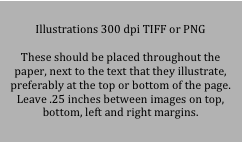
\includegraphics[width=3.31in]{figure.png}
% \caption{This is an example of figure caption. Note that all figures, and tables are to be referenced in the text. \copyright Respect Copyright.}
% \end{figure}

% \begin{figure*}
% 
\includegraphics[width=\textwidth]{two-column-figure.png}
% \caption{Example of a double-column figure with caption. \copyright Respect Copyright.}
% \end{figure*}

% \begin{quote}
%     Art as we name and understand it in our societies — Art in the singular, with a capital A — was unknown to those who enjoyed themselves at the theatre, commissioned works from painters and sculptors, listened to religious concerts, or hired musicians for their feasts or ceremonies. This is not a merely lexical issue. Art did not exist as a common sphere of experience, not only because the practice of the arts was intended for different social purposes, but, above all, because these purposes were themselves part of a hierarchical division of human activities and of the human beings who engaged in them. \citep[p.25]{RanciereMdrnTms2022}
% \end{quote}

% The regime of representation is epitomised for Rancière by classical theatre, in which the two meanings of the word sense — sensing as in experiencing, and making sense as in to understand conceptually — are tightly coupled.

% \begin{quote}
%     The stage was thought of as a magnifying mirror where spectators could see the virtues and vices of their fellow human beings in fictional form. And that vision in turn was supposed to prompt specific changes in their minds: Molière’s Tartuffe supposedly taught spectators to recognize hypocrites; Voltaire’s Mahomet to fight for tolerance against fanaticism, and so on. Now, that ability to produce the dual effect of intellectual recognition and appropriate emotion was itself predicated on a regime of concordance inherent in representation.
% \end{quote}

% Art “as technics“, Sauvagnargues says, “concerns the way in which materials (matières) are captured and assembled into matter (matière) of expression.” \citep[p.75]{SauvagnarguesArtmchns2016}. However, art is not reducible to technics so that it does not require a specific kind of analysis \citep[p.74]{SauvagnarguesArtmchns2016}.

% An effective theory is one that is “able to organize phenomena under an efficient set of principles” and is also “not impossibly complex” \citep[p.1]{WellsEffctvThrs2012}. A good effective theory functions as a heuristic — a rule of thumb that can serve as a guide for action. The critical requirement is \emph{observational consistency} (an effective theory need not be even be true, as long as it works) \citep[p.71]{WellsEffctvThrs2012}.

% Flack has referred to an earlier study in which she worked with a group of monkeys (pigtailed macaques) who used a silent, bared-teeth signal to communicate about their specific position in a power distribution, as if each individual monkey had a “power score”. The power score was a “course-grained representation of [...] an individual's fighting ability as collectively perceived by the group” \citep[p.5]{FlackCrsGrnng2017}. The power distribution was very stable\footnote{

%     During the study there was only one relationship reversal over the course of 5 months. \citep[p.1584]{FlackCntxtMdltsSgnlMnng2007}

% }. This silent bared-teeth signal was always used in interactions between only two monkeys and was only emitted by the monkey with a lower power score. Flack found that the signal occurred in two contexts:

% \begin{enumerate}
%     \item{
%         In response to aggression or threat of it
%     }
%     \item{
%         During pass-bys and approaches in the absence of any overt aggression or threatening behavior
%     }
% \end{enumerate}

% The first use case, when the signal was used during conflict, can be read in behaviourist terms as a simple stimulus response. In this case the signal functioned as an indicator of submission. Flack focused instead on the use of the signal during peaceful encounters and found that its use was always correlated with the position in the power distribution of each monkey. She has suggested that the signal, when used in this context “enabled communication about subordination, a pattern of behavior, rather than just submission in the present interaction” \citep[p.1584]{FlackCntxtMdltsSgnlMnng2007}.

% The pattern of power distribution within the social system of the monkeys was apparently functioning as a store of information about the relative capability of each monkey to win fights\footnote{

%     Presumably fighting ability correlates with some fitness parameters

% }. The signalling process was making the information available in an easy, low-energy (coarse-grained) form. There was no need for the monkeys to be constantly fighting in order to know where they are positioned, nor to remember the power distribution (to store it in their brain). A monkey only needed to maintain an awareness of their power score, which they gleaned from casual interactions and from watching the interactions of other monkeys\footnote{

%     The power score is not a number (of course) but an estimate of “the \emph{degree of consensus} in the group that they can win fights” \citep[p.5]{FlackCrsGrnng2017}.

% }. The stable power distribution, as it was continually reinforced through the network of interactions and signals, made possible otherwise costly conflict-management strategies, such as a kind of policing strategy in which the most powerful monkeys were unchallenged when they intervened to break up disputes \citep[p.5]{FlackCrsGrnng2017}.

% If Flack's distinction between \emph{coarse-graining in Nature} and \emph{coarse-graining by scientists} is valid, it would make the concept less useful. Addressing an imagined readership of scientists, Flack referred to ideas like temperature as “coarse-grainings that we as scientists impose on the system to find compact descriptions of system behaviour sufficient for good prediction.” In making a distinction between what scientists do and “how adaptive systems identify regularities and build effective theories to guide adaptive decision-making and behaviour”, Flack was apparently suggesting, or assuming, that communities of scientists working together to measure and observe phenomena are somehow not \emph{adaptive systems identifying regularities and building effective theories to guide adaptive decision-making and behavior}. Clearly they are, as Chang, Latour and Woolgar, and other philosophers and historians of science have shown\footnote{
    
%     See DeLanda's discussion of the way scientists produce theories, e.g. he quotes Alan Garfinkel (Forms of Explanation, pp. 53–8): “an object of explanation should be chosen which is stable under small perturbations of its conditions.” \citep[pp.161-162]{DeLandaIntnsvSci2013}

% }.

% Coarse-graining is a more useful concept if it is not divided into two different types, one for scientists and one for the rest of reality. Scientists are participants in a complex process that includes, depending on where one decides to draw the boundary, the full human and social context of particular scientists, science itself, various technologies, the phenomena under observation and even quantum entanglements. Flack's tendency to treat science as something separate from nature could perhaps be an example of course-graining. She has noted that components in a complex system can tune to a slow variable regardless of whether it actually does a good job of summarizing regularities. “Think”, she has advised us, ”of social institutions that are highly constraining and very hard to change” \citep[p.9]{FlackCrsGrnng2017}.

% In any case, those days are over.

% The American critic and philosopher of art Arthur Danto was one of the first to point out the absurdity of the idea that aesthetic experiences are synonymous with the experiences of beauty (and also that it is a kind of philosophical colonialism, since it requires a single subjective, culturally informed, experience to function as an objective definition \citep[p.124]{DantoEmbdMnngs2007}), and that a focus on beauty has had the effect of delegitimising the real diversity of aesthetic experiences artists routinely deploy \citep[p.59]{DantoThAbsOfBty2003}, which might be based in virtually any kind of observed quality, like cuteness \citep[p.28]{DantoThPhlsphclArt2005}, grunge, blandness \citep[p.126]{DantoEmbdMnngs2007}, disgustingness, eroticism, \citep[p.59]{DantoThAbsOfBty2003}, et cetera.

% A final example is Frank Stella's 1959 stripe paining \emph{The Marriage of Reason and Squalor II}. Which

% \begin{quote}
%     [...] appears to be as resolutely determinate and definite as a painting can be, a kind of no-nonsense record of the process of its own creation. The painting is simultaneously composed of, and comprises, two sets of twelve equally spaced and concentrically organized stripes, each of which is a flat uninflected brushstroke the width of the brush with which it was painted.
% \end{quote}

% Stella apparently described his goals for the painting in blunt terms as being to “keep the paint as good as it was in the can” \citep[p.38]{HoelscherArtAsInfrmtn2021}. He also said of it: “What you see is what you see” \citep[p.39]{HoelscherArtAsInfrmtn2021}. However, Hoelscher has suggested, the painting is not as simple as it appears.

% \begin{quote}
%     [...] By the time Stella painted his first stripe paintings in 1959, art's network of discursive entanglements had reached a state so charged with potential that it was able to produce artworks discursively coded as nondiscursive objects [...] each painting has been discursively coded as a simple and nondiscursive object, the simple nondiscursivity of which makes it discursively important according to a complex weave of artistic discourses built up over the course of a century.
% \end{quote}

% Hoelscher summed up the operation of Stella's painting in the same informational terms as the Morris sculpture and the Duchamp readymade.

% \begin{quote}
%     Enfolding multiple orders of operation that range from deadpan brushstrokes, to objecthood, to tautological statement, to large-scale discursive and cultural complexes of ideas, the Stella stripe painting + statement ensemble thus operates as a differential object, as a bundle of tightly entangled yet irresolvable differences that propagate still further difference.
% \end{quote}

% In the early 2000s, the mode of resonance between philosophical and scientific theories of complexity found conceptual form in the term \emph{complexity thinking}, which started to be used by scholars and practitioners working in fields like management theory, organisational change, health and education. At this time, Complex Adaptive Systems theory was filtering through into popular culture with memes like “chaos theory” and the concept of \emph{emergence} capturing the collective imagination. The term \emph{complexity thinking} expresses a sense of complexity as an intrinsic quality shared by diverse phenomena, and a sense of things being connected in unpredictable ways. The term acknowledges, according to Paul Cilliers and Kurt Richardson, the “...epistemological consequences of assuming the ubiquity of complexity” \citep{CilliersRichardsonCmplxtyScnc2001}. Complexity thinking describes an awareness that we can never fully know the dynamic interconnected processes at play within and between all phenomena. While it limits what we can reasonably claim to know, it also changes how we think about the world in ways that create new possibilities for knowing. 